\documentclass{TDP003mall}

\newcommand{\version}{Version 1.2}
\author{Alexander Jonsson, \url{alejo720@student.liu.se}\\
  Joakim Johansson, \url{joajo229@student.liu.se}}
\title{Designspecifikation}
\date{2016-12-17}
\rhead{Alexander Jonsson \\
Joakim Johansson}

\usepackage{float}
\usepackage{listings}
\usepackage{color}

\begin{document}
\projectpage

\tableofcontents

\newpage

\section{Revisionshistorik}
\begin{table}[!h]
\begin{tabularx}{\linewidth}{|l|X|l|}
\hline
Ver. & Revisionsbeskrivning & Datum \\\hline
1.2 & Uppdaterat klassdiagram och detaljbeskrivning, samt korrekturläst & 2016-12-17 \\\hline
1.1 & Lagt till detaljbeskrivning. & 2016-11-30 \\\hline
1.0 & Första utkast med klassdiagram, externa filer samt diskussion om valet av design. & 2016-11-25 \\\hline
\end{tabularx}
\end{table}

\newpage

\section{UML klassdiagram av systemet}
Här visas ett UML klassdiagram för den logiska delen av systemet:
\begin{figure}[H]
    \centering
    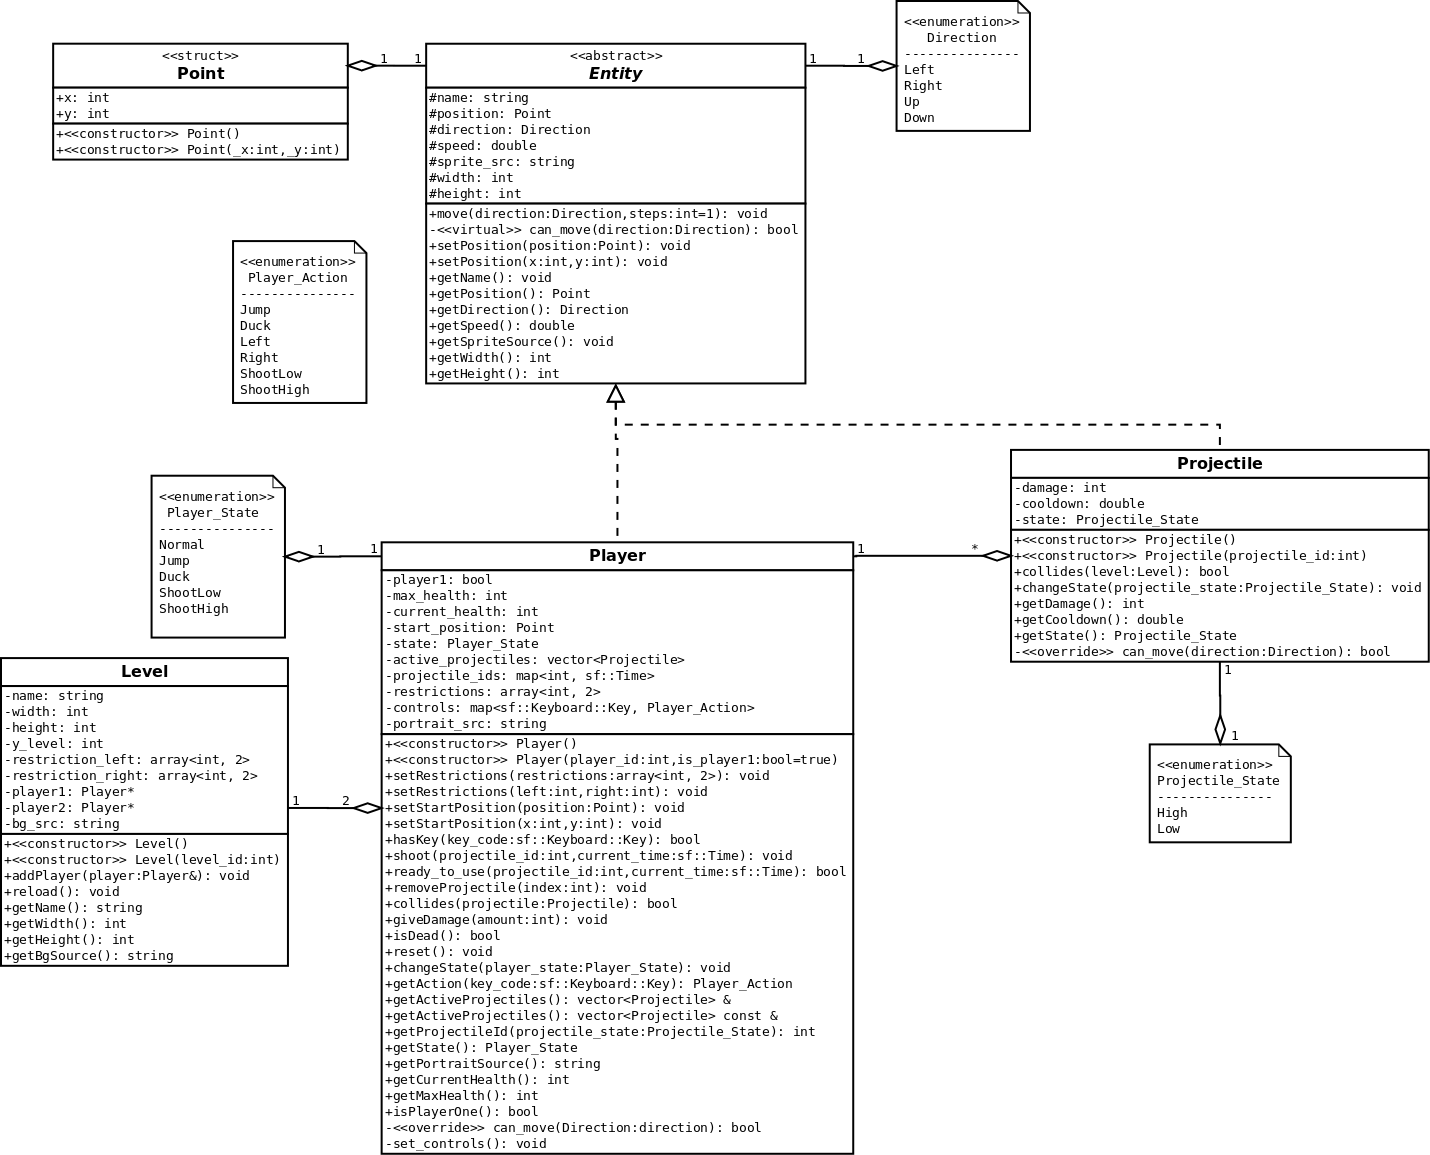
\includegraphics[width = \linewidth]{classdiagram_logic.png}
    \caption{Klassdiagram: logisk del}
    \label{fig:classdiagraM_logic}
\end{figure}

\newpage

Här visas ett UML klassdiagram för den grafiska delen av systemet:
\begin{figure}[H]
    \centering
    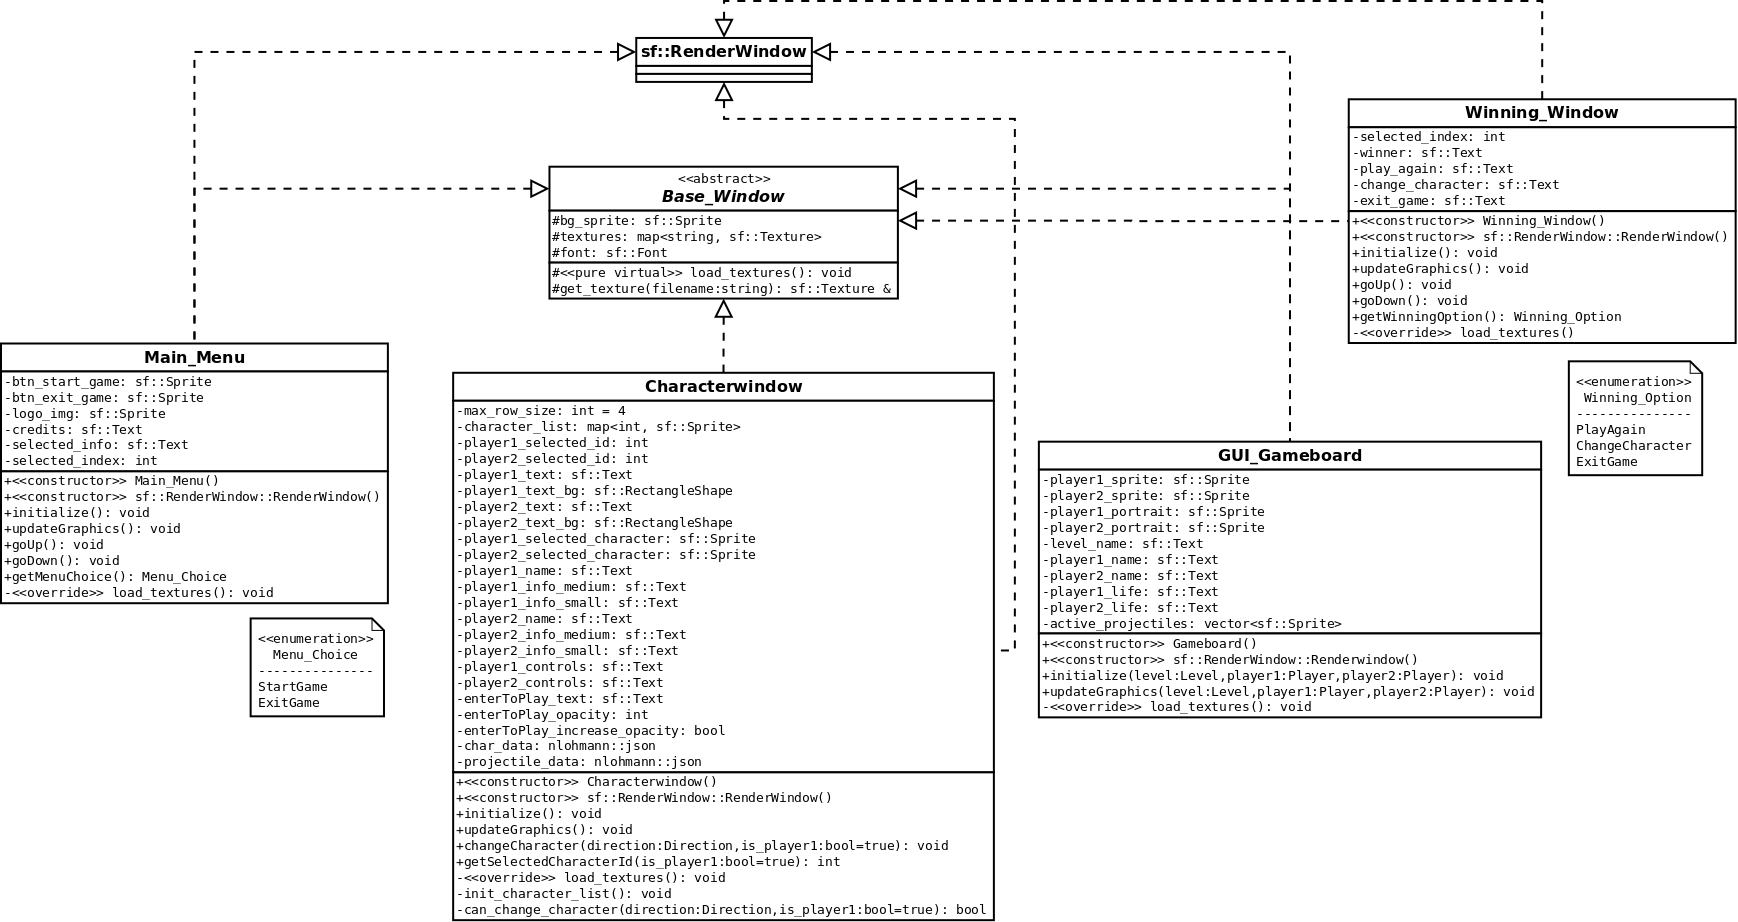
\includegraphics[width = \linewidth]{classdiagram_gui.png}
    \caption{Klassdiagram: grafisk del}
    \label{fig:classdiagram_gui}
\end{figure}

\newpage

Här visas ett UML klassdiagram för huvud klassen som representerar själva spelet:
\begin{figure}[H]
	\centering
	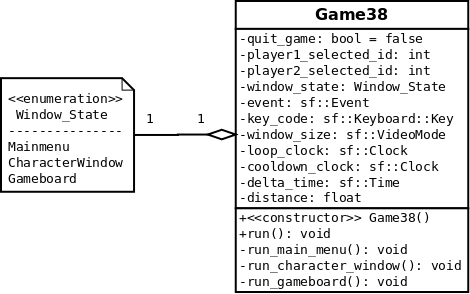
\includegraphics[width = \linewidth]{classdiagram_game.png}
	\caption{Klassdiagram: spelklassen}
	\label{fig:classdiagram_game}
\end{figure}

\newpage

\section{Detaljbeskrivning}
\subsection{Player}
• \textbf{Namn:} \\
\indent- Player (spelare) \\
• \textbf{Syfte:} \\
\indent- Syftet med klassen 'Player' är att ha en mall som representerar en spelare med olika egenskaper.
\\
• \textbf{Relationer:} \\
\indent- Denna klass ärver från en 'Entity'-klass. \\
\indent- Klassen 'Level' hanterar två spelare (spelare 1 och 2). \\
\indent- Denna klass äger och hanterar 'Projectile'-objekt. \\
• \textbf{Konstruktor:} \\
\indent- Klassen har en konstruktor som tar in ett ID och om det är spelare 1 eller inte. Sedan används ID:t till att hämta korrekt data från JSON-filen innehållande karaktärdatan. Spelarens kontroller sätts även beroende på om det är spelare ett eller inte \\
• \textbf{Publika metoder:} \\
\indent- \textbf{hasKey(keycode)}: Kollar om den specificerade knappen är en knapp spelaren kan använda. \\
\indent- \textbf{shoot(projectile\_id, current\_time):} Skapar en projektil beroende på vilket ID och lägger in den i listan med spelarens projektiler. Samtidigt läggs nuvarande tid på i listan med spelarens projektil-id:n. \\
\indent \textbf{readyToUse(projectile\_id, current\_time)} Kollar om projektilen med den specificerade projektil-id:t kan användes beroende på hur långt tid som gått sedan senaste användningen av projektilen. \\
\indent \textbf{removeProjectile(index)} Tar bort en spelares projektil beroende på position i listan med aktiva projektiler \\
\indent- \textbf{collides(projectile):} Kollar om spelaren kolliderar med den specificerade projektilen. \\
\indent- \textbf{giveDamage(amount):} Minskar spelarens liv med den specificerade mängden. \\
\indent- \textbf{isDead():} Kollar om spelarens liv är noll.\\
\indent- \textbf{reset():} Flyttar t.ex. spelaren till spelarens startposition, ger spelaren fullt liv och tar bort alla ägda projektiler från spelaren.\\
\indent- \textbf{move(direction, steps)}: Flyttar spelaren ett specificerat antal steg åt den specificerade riktningen tills det inte är möjligt längre. \\
• \textbf{Variabler:} \\
\indent- \textbf{position:} Håller reda på spelarens nuvarande position. \\
\indent- \textbf{direction:} Håller reda på vilket håll spelaren är vänd åt. \\
\indent- \textbf{speed:} Håller reda på hur snabbt spelaren kan röra sig. \\
\indent- \textbf{sprite\_src:} Filnamnet på spelarens textur. \\
\indent- \textbf{portrait\_src:} Filnamnet på spelarens porträttbild. \\
\indent- \textbf{width:} Spelarens bred. \\
\indent- \textbf{height:} Spelarens höjd. \\
\indent- \textbf{name:} Namnet på karaktären spelaren har valt. \\
\indent- \textbf{player1:} Håller reda på om spelaren är spelare 1 eller 2. \\
\indent- \textbf{max\_health:} Maximala mängden liv spelarens karaktär kan ha. \\
\indent- \textbf{health:} Nuvarande mängden liv spelaren har. \\
\indent- \textbf{start\_position:} Position spelaren ska start på, i detta fall på spelplanen. \\
\indent- \textbf{state:} Håller reda på vilket tillstånd spelaren är i (Hoppa, ducka eller stående). \\
\indent- \textbf{active\_projectiles:} En lista med projektiler spelaren skjuter just nu. \\
\indent- \textbf{projectile\_ids:} En lista med ID:n på projektiler som spelaren kan använda. \\
\indent- \textbf{restrictions:} Definierar ett område spelaren kan röra sig inom, i detta fall på spelplanen. \\
\indent- \textbf{controls}: En tabell på vilka knappar som leder till vilken spelarhandling. \\

\newpage

\subsection{Level}
• \textbf{Namn:} \\
\indent- Level (nivå) \\
• \textbf{Syfte:} \\
\indent- Syftet med klassen 'Level' är att ha en mall som representerar en spelplan med olika egenskaper.
\\
• \textbf{Relationer:} \\
\indent- Denna klass äger två spelare: ('Player'-klasser) spelare 1 och 2. \\
• \textbf{Konstruktor:} \\
\indent- Klassen har en konstruktor som tar in ett ID. Sedan används ID:t till att hämta korrekt data från JSON-filen innehållande nivådatan. \\
• \textbf{Publika metoder:} \\
\indent- \textbf{addPlayer(player):} Lägger till en spelare till spelplanen och lagras i spelare 1 eller 2 beroende på vad den specificerade spelaren är. \\
\indent- \textbf{reload():} Återställer spelplanen och alla objekt på den. \\
• \textbf{Variabler:} \\
\indent- \textbf{name:} Namnet på nivån. \\
\indent- \textbf{width:} Bredden på nivån. \\
\indent- \textbf{height:} Höjden på nivån. \\
\indent- \textbf{y\_level:} Bestämmer hur högt spelarna står ifrån botten av nivån. \\
\indent- \textbf{restriction\_left:} Definierar vänstra planhalvan. \\
\indent- \textbf{restriction\_right:} Definierar högra planhalvan. \\
\indent- \textbf{player1:} Spelare 1 på spelplanen. \\
\indent- \textbf{player2:} Spelare 2 på spelplanen. \\
\indent- \textbf{bg\_src:} Filnamn på nivåns bakgrundsbild. \\

\section{Diskussion av valet om design}
\subsection{Fördelar}
• Klasser ärver andra klasser. Exempelvis ärver 'Player' och 'Projectile'-klasserna utav 'Entity'-klassen vilket leder till återanvändning av kod. Det gör det även lättare att skapa en liknande klass senare.
\\ \\
• De grafiska klasserna innehåller endast grafiska komponenter vilket leder till separation mellan det grafiska och logiska. Detta gör det möjligt att det grafiska eller logiska ska kunna användas till andra system.
\\ \\
• Att läsa objekts egenskaper från filer leder till mindre kod då vi slipper hårdkoda objektens egenskaper inuti koden.
\subsection{Nackdelar}
• Alla grafiska klasser som representerar ett fönster ärver både från en 'Base\_Window' och 'sf::RenderWindow' klassen. Eftersom 'Base\_Window' ska representera ett fönster skulle det ha varit med lämpligt att endast 'Base\_Window' ärvde från 'sf::RenderWindow'. Detta skulle skapa en smidigare klassstruktur.
\\ \\
• I spelarobjektet lagras det internt om spelaren är spelare 1 eller 2. Detta begränsar spelarklassen ifall det skulle behövas fler än två spelare.

\newpage

\section{Externa filer}
\subsection{Mappstruktur}
\begin{lstlisting}[backgroundcolor = \color{lightgray}]
resources
    img
        level
            *_portrait.png
            *.png
        character
            *_portrait.png
            *.png
        projectile
            *.png
    data
        levels.json
        characters.json
        projectiles.json
        *.json
    music
        *.mp3
    sfx
        *.wav
*.cc
*.h
settings.config
\end{lstlisting}
I 'root'-mappen ligger alla 'C++'-filer, konfigurationsfiler och en mapp som innehåller alla statiska filer som spelet ska ladda information från. Exempel på denna information är bilder, musik, ljudfiler och data som krävs för de olika objekten. '*\_portrait'-bilderna är de bilder som ska visas vid val av karaktär. Alla data filer som ska användas är i 'JSON'-format vilket kräver att vi laddar ner en modul för att hantera 'JSON'-filer i C++.

\newpage

\subsection{Nivåer}
Detta är ett exempel på hur en 'JSON'-fil innehållandes de olika nivåernas data skulle kunna se ut:
\begin{lstlisting}[backgroundcolor = \color{lightgray}]
[
    {
        "id": 1,
        "name": "Avalanche Leftovers",
        "width": 800,
        "height": 640,
        "y_level": 100,
        "restriction_left": [20, 350],
        "restriction_right": [400, 780],
        "bg_src": "avalanche_leftovers.png",
        "portrait_src": "avalanche_leftovers_portrait.png",
        "music": "icy_wind.wav"
    },
    {
        "id": 2,
        "name": "Firelands",
        "width": 1024,
        "height": 1280,
        "y_level": 20,
        "restriction_left": [100, 200],
        "restriction_right": [824, 924],
        "bg_src": "firelands.png",
        "portrait_src": "firelands_portrait.png",
        "music": "scorching_battle.wav"
    }
]
\end{lstlisting}

\newpage

\subsection{Karaktärerer}
Detta är ett exempel på hur en 'JSON'-fil innehållandes de olika karaktärernas data skulle kunna se ut:
\begin{lstlisting}[backgroundcolor = \color{lightgray}]
[
	{
		"id": 1,
		"name": "Crazy guy",
		"width": 190,
		"height": 220,
		"max_health": 1000,
		"speed": 1.2,
		"projectiles": [1, 2],      
		"sprite_src": "crazy_guy.png",
		"portrait_src": "crazy_guy_portrait.png"
	},
	{
		"id": 2,
		"name": "Less crazy guy",
		"width": 190,
		"height": 220,
		"max_health": 750,
		"speed": 1.5,
		"projectiles": [3, 4],
		"sprite_src": "less_crazy_guy.png",
		"portrait_src": "less_crazy_guy_portrait.png"
	}
]
\end{lstlisting}

\newpage

\subsection{Projektiler}
Detta är ett exempel på hur en 'JSON'-fil innehållandes de olika projektilernas data skulle kunna se ut:
\begin{lstlisting}[backgroundcolor = \color{lightgray}]
[
	{
		"id": 1,
		"name": "Football",
		"state": "low",
		"width": 40,
		"height": 40,
		"damage": 25,
		"speed": 3.0,
		"sprite_src": "football.png",
		"cooldown": 0.3
	},
	{
		"id": 2,
		"name": "Mountain Dew",
		"state": "high",
		"width": 40,
		"height": 40,
		"damage": 100,
		"speed": 1.0,
		"sprite_src": "mountain_dew.png",
		"cooldown": 1
	},
	{
		"id": 3,
		"name": "BOMB",
		"state": "high",
		"width": 40,
		"height": 40,
		"damage": 450,
		"speed": 0.3,
		"sprite_src": "bomb.png",
		"cooldown": 5
	},
	{
		"id": 4,
		"name": "Nut",
		"state": "low",
		"width": 40,
		"height": 40,
		"damage": 7,
		"speed": 2,
		"sprite_src": "nut.png",
		"cooldown": 0.1
	}
]
\end{lstlisting}

\newpage

\subsection{Konfigurationsfil}
Detta är exempel på hur strukturen i konfigurationsfilen skulle kunna se ut:
\begin{lstlisting}[backgroundcolor = \color{lightgray}]
player1_jump 'w'
player1_left 'a'
player1_duck 's'
player1_right 'd'
player1_low_shoot 'r'
player1_high_shoot 't'
player2_jump 'up-arrow'
player2_left 'left-arrow'
player2_duck 'down-arrow'
player2_right 'right-arrow'
player2_low_shoot 'o'
player2_high_shoot 'p'
\end{lstlisting}


\end{document}
